\documentclass[aspectratio=169,11pt]{beamer}
\usepackage[T1]{fontenc}
\usepackage[utf8]{inputenc}
\usepackage{lmodern,amsmath,booktabs}
\graphicspath{{figures/backtest/}}

\definecolor{Accent}{HTML}{007A75}
\setbeamercolor{structure}{fg=Accent}
\setbeamercolor{frametitle}{fg=white,bg=Accent}
\setbeamertemplate{navigation symbols}{}

\newcommand{\VaR}{\operatorname{VaR}}
\newcommand{\ES}{\operatorname{ES}}
\newcommand{\CE}{\operatorname{CE}}
\newcommand{\ind}{\mathbf{1}}
\newcommand{\source}[2]{\vfill{\scriptsize\href{#1}{#2}}}

\begin{document}

% ------------------------------------------------------------ model (1)
\begin{frame}{Model łącznego rozkładu stóp zwrotu}

\begin{block}{Rozkłady brzegowe: AR(1)--GJR-GARCH(1,1) ze skośnym \(t\)}
\[
  r_t=\mu+\phi\,r_{t-1}+\sigma_t z_t,\quad
  \sigma_t^2=\omega+\bigl(\alpha+\delta\,\ind\{\varepsilon_{t-1}<0\}\bigr)
    \varepsilon_{t-1}^2+\beta\,\sigma_{t-1}^2,\quad
  z_t\sim\text{skew-}t(\eta,\lambda).
\]
\end{block}

\begin{block}{Zależność: kopuła R-vine na pseudoobserwacjach reszt}
\[
  c(u_1,\ldots,u_d)=\prod_{\ell=1}^{L}\prod_{e\in T_\ell}
    c_{a_e b_e\mid D_e}\bigl(F(u_{a_e}\mid u_{D_e}),\,F(u_{b_e}\mid u_{D_e})\bigr).
\]
\end{block}

{\small
Estymacja w oknie 1260 sesji przed datą decyzji; \(\delta>0\) oznacza
silniejszy wzrost zmienności po spadkach. Kopułę dopasowujemy do
\(\hat u_{i,t}=\operatorname{rank}(s_{i,t})/(n+1)\), gdzie
\(s_{i,t}=\sum_{j=0}^{4}\hat z_{i,t-j}\) uwzględnia niesynchroniczne
notowania GPW, NYSE i NBP. R-vine (\(L=3\) drzewa) porównujemy m.in.\
z kopułą gaussowską i \(t\).
}

\source{https://github.com/michalmarchwiak/bsc-project/blob/main/docs/dependence_model.md}
       {Model zależności: docs/dependence\_model.md}
\end{frame}

% ------------------------------------------------------------ pasted (1)
\begin{frame}{Od scenariuszy Monte Carlo do ryzyka funduszu}

Dla każdej daty rebalansowania symulujemy wspólne stopy zwrotu
aktywów w PLN na horyzont 21 sesji. Każdy scenariusz daje jedną
stopę zwrotu całego funduszu.

\[
  L_s = -\sum_{i=1}^{d} w_i R_{s,i},
  \qquad s=1,\ldots,N.
\]

{\small
\(R_{s,i}\) to stopa zwrotu instrumentu \(i\) w scenariuszu \(s\),
a \(w_i\) to jego udział w całym funduszu.
}

\begin{block}{Co odczytujemy z rozkładu strat?}
\begin{itemize}
  \item \textbf{VaR 97,5\%} wyznacza próg przekraczany
        w około 2,5\% scenariuszy.
  \item \textbf{ES 97,5\%} to średnia strata
        w najgorszych 2,5\% scenariuszy.
\end{itemize}
\end{block}

Liczbę scenariuszy zwiększamy partiami, aż oszacowanie ES
dla portfeli kontrolnych osiągnie wymaganą precyzję
lub dojdziemy do limitu symulacji.

\source{https://github.com/michalmarchwiak/bsc-project/blob/main/docs/backtest.md}
       {Metodologia projektu, sekcja 4}
\end{frame}

% ------------------------------------------------------------ model (2)
\begin{frame}{Funkcja celu i ograniczenie look-through}
\small

\begin{block}{Ekwiwalent pewności z karą za wspólne spadki}
\[
  \max_{w}\ \CE_\gamma(w)-\kappa\,\sigma^{EW}\,w^{\mathsf T}\Lambda(q)\,w,
  \qquad
  \CE_\gamma(w)=\Bigl(\tfrac1N\sum_{s=1}^{N}
    (1+R_s^{\mathsf T}w)^{1-\gamma}\Bigr)^{\frac{1}{1-\gamma}}-1,
\]
\[
  \Lambda_{ij}(q)=\tfrac{1}{Nq}\textstyle\sum_{s=1}^{N}
    \ind\{V_{s,i}\le q\}\,\ind\{V_{s,j}\le q\},\qquad q=0{,}05 .
\]
\end{block}

\begin{block}{Dwa poziomy i limit ekspozycji na instrument}
\[
  x_i=W_k\,w_{k,i}\le c_{LT}
  \iff
  W_k\le u_k=\min\Bigl(W_{\max},\ \frac{c_{LT}}{\max_i w^*_{k,i}}\Bigr).
\]
\end{block}

{\small
\(\gamma\) -- awersja do ryzyka, \(\kappa\) -- waga kary, \(\Lambda_{ij}\)
szacuje \(P(V_j\le q\mid V_i\le q)\). Najpierw wyznaczamy \(w_k^*\) w subfunduszach,
potem wagi subfunduszy \(W\) przy \(0\le W_k\le u_k\).
Funkcja celu jest wklęsła, więc optimum jest globalne.
}

\source{https://github.com/michalmarchwiak/bsc-project/blob/main/docs/backtest.md}
       {Metodologia projektu, sekcja 5}
\end{frame}

% ------------------------------------------------------------ pasted (2)
\begin{frame}{Jak wykorzystujemy ryzyko do wyboru wag?}

Najpierw dobieramy wagi instrumentów wewnątrz subfunduszy.
Następnie ustalamy udziały subfunduszy w całym portfelu.

\begin{block}{Przykład: strategia minimalnego ES}
Dla zadanych scenariuszy szukamy wag, przy których średnia
strata w najgorszej części rozkładu jest najmniejsza.
Problem można zapisać jako program liniowy:
\[
\begin{aligned}
\min_{w,z,u}\quad &
   z+\frac{1}{N(1-\alpha)}\sum_{s=1}^{N}u_s \\[2pt]
\text{przy}\quad &
   u_s\ge -R_s^{\mathsf T}w-z,\quad u_s\ge0
   &&(s=1,\ldots,N),\\
&  \sum_{i=1}^{d}w_i=1,\quad 0\le w_i\le \overline w_i
   &&(i=1,\ldots,d).
\end{aligned}
\]
\end{block}

{\small
\(z\) jest progiem straty, a \(u_s\) opisuje jej nadwyżkę ponad
próg. Wyniki strategii porównujemy m.in. z portfelem równoważonym.
}

\source{https://github.com/michalmarchwiak/bsc-project/blob/main/docs/backtest.md}
       {Metodologia projektu, sekcja 5}
\end{frame}

% ------------------------------------------------------------ wykresy
\begin{frame}{Skład subfunduszy w czasie}
\centering
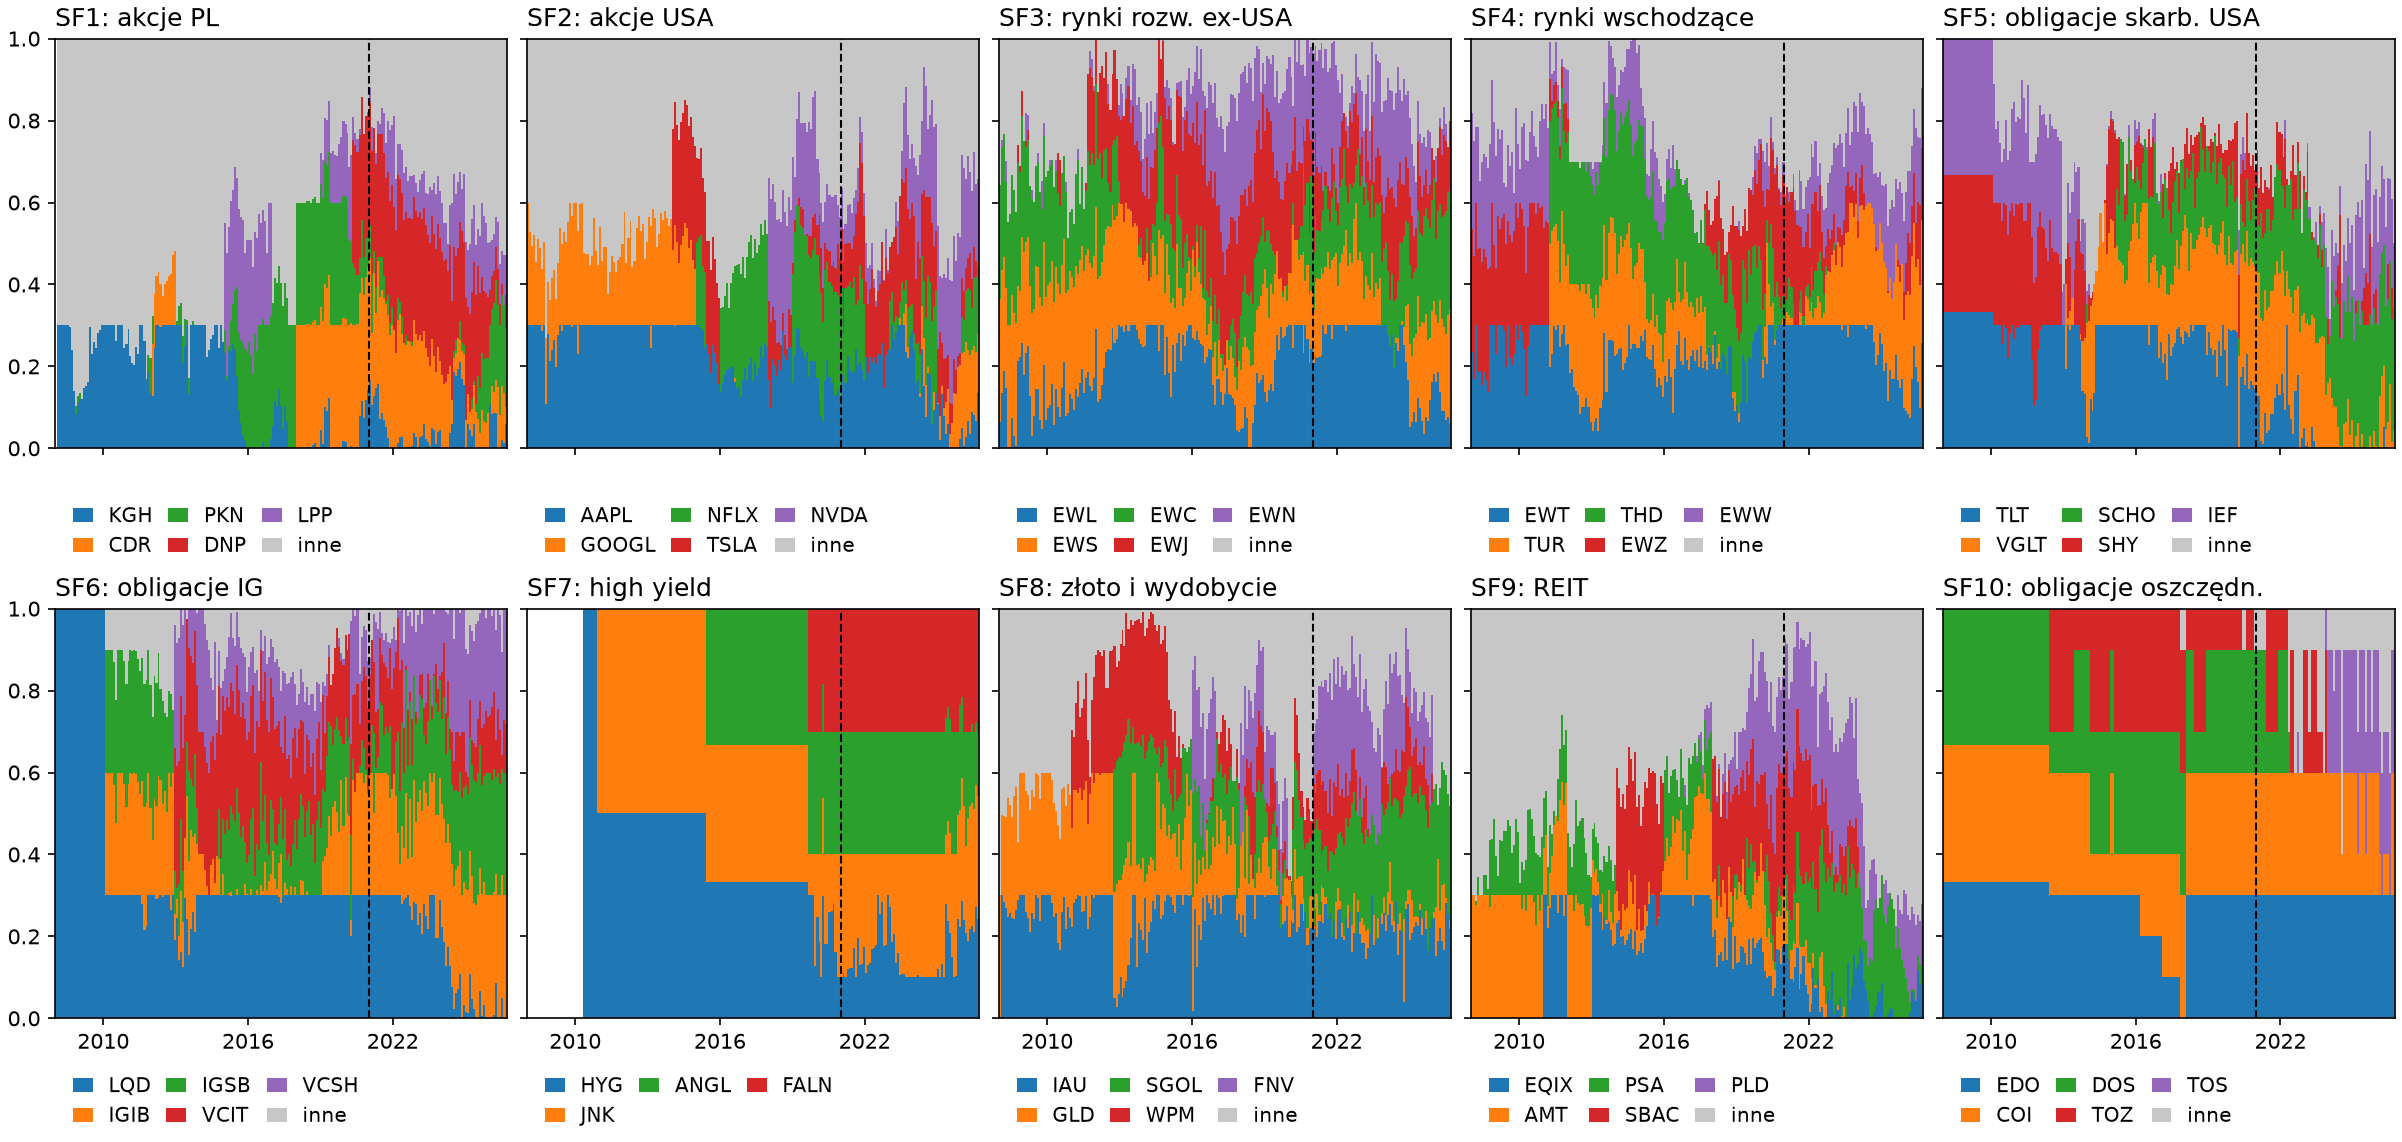
\includegraphics[width=\textwidth,height=.68\textheight,keepaspectratio]{subfund_composition_P3.png}\par
{\scriptsize Wagi \(w_{k,i}\) w subfunduszach, R-vine \(\times\) \texttt{ce\_dep},
  profil P3; 5 instrumentów o największej średniej wadze, reszta jako „inne”;
  linia przerywana: początek hold-outu.}
\source{https://github.com/michalmarchwiak/bsc-project/blob/main/pipelines/composition_figures.py}
       {Kod wykresu: pipelines/composition\_figures.py}
\end{frame}

\begin{frame}{Skład portfela w czasie: profile P1--P3}
\centering
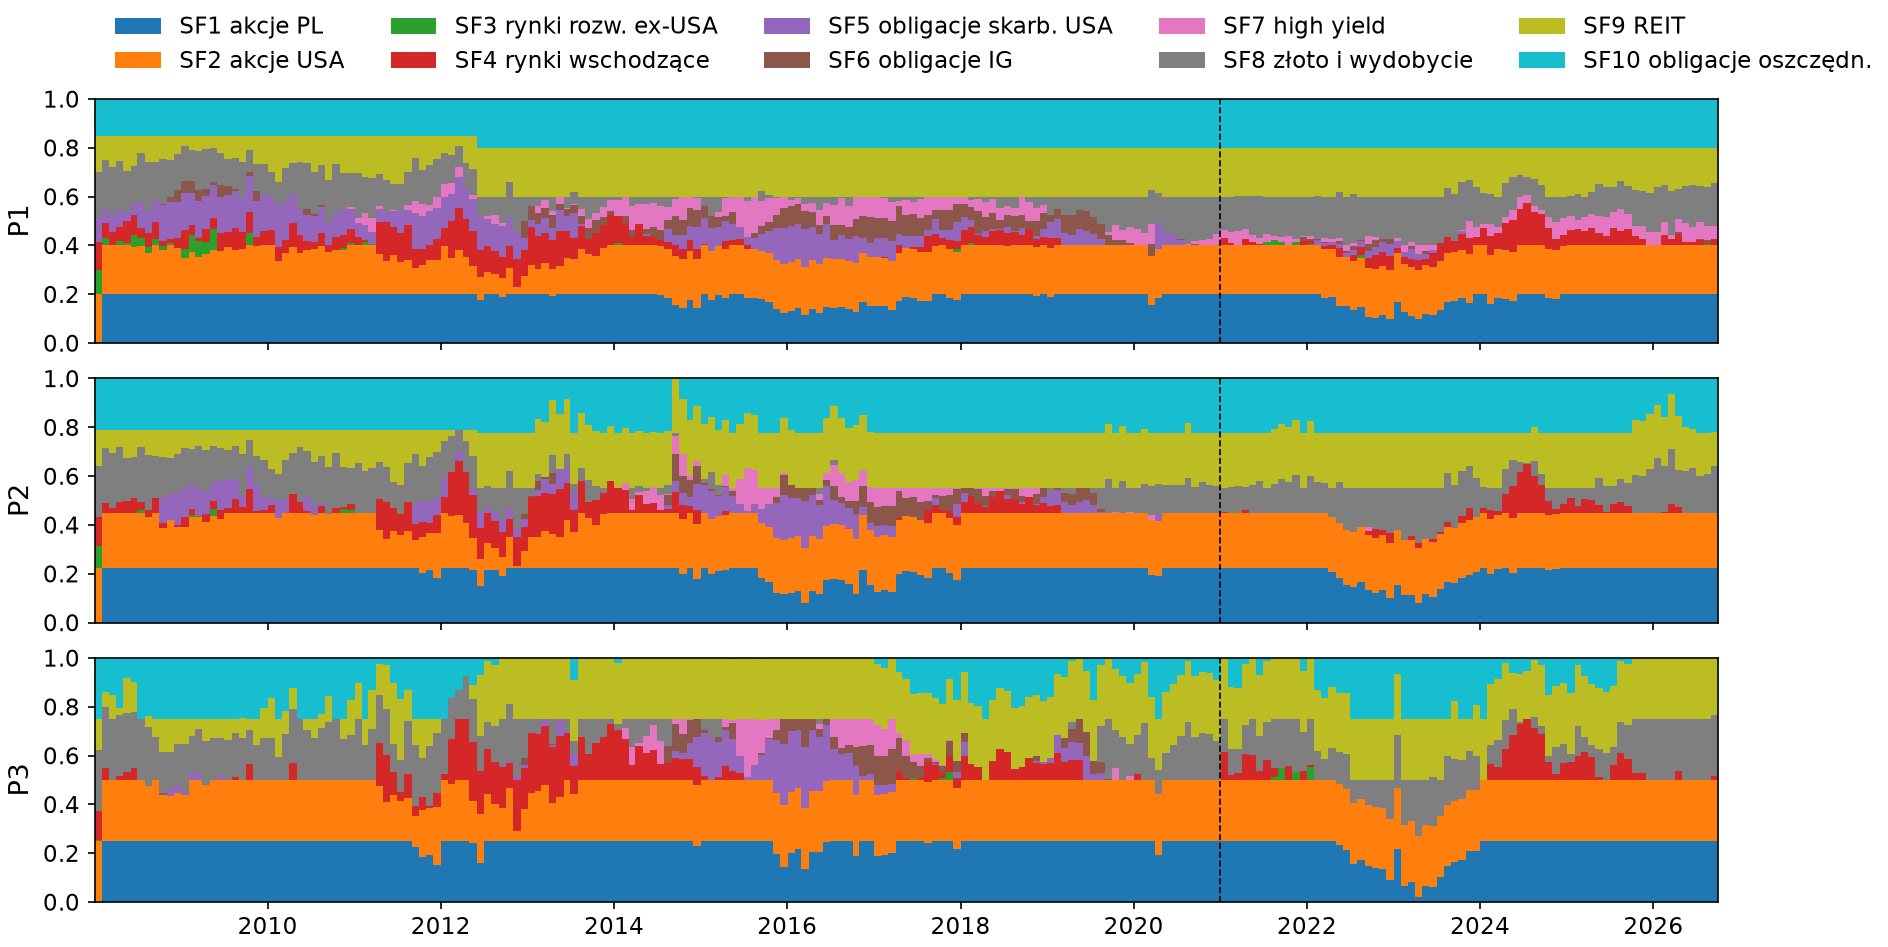
\includegraphics[width=\textwidth,height=.74\textheight,keepaspectratio]{portfolio_W_P1-P3.png}\par
{\scriptsize Wagi subfunduszy \(W_k\), R-vine \(\times\) \texttt{ce\_dep};
  linia przerywana: początek hold-outu.}
\source{https://github.com/michalmarchwiak/bsc-project/blob/main/pipelines/composition_figures.py}
       {Kod wykresu: pipelines/composition\_figures.py}
\end{frame}

\begin{frame}{Skład portfela w czasie: profile P4--P5}
\centering
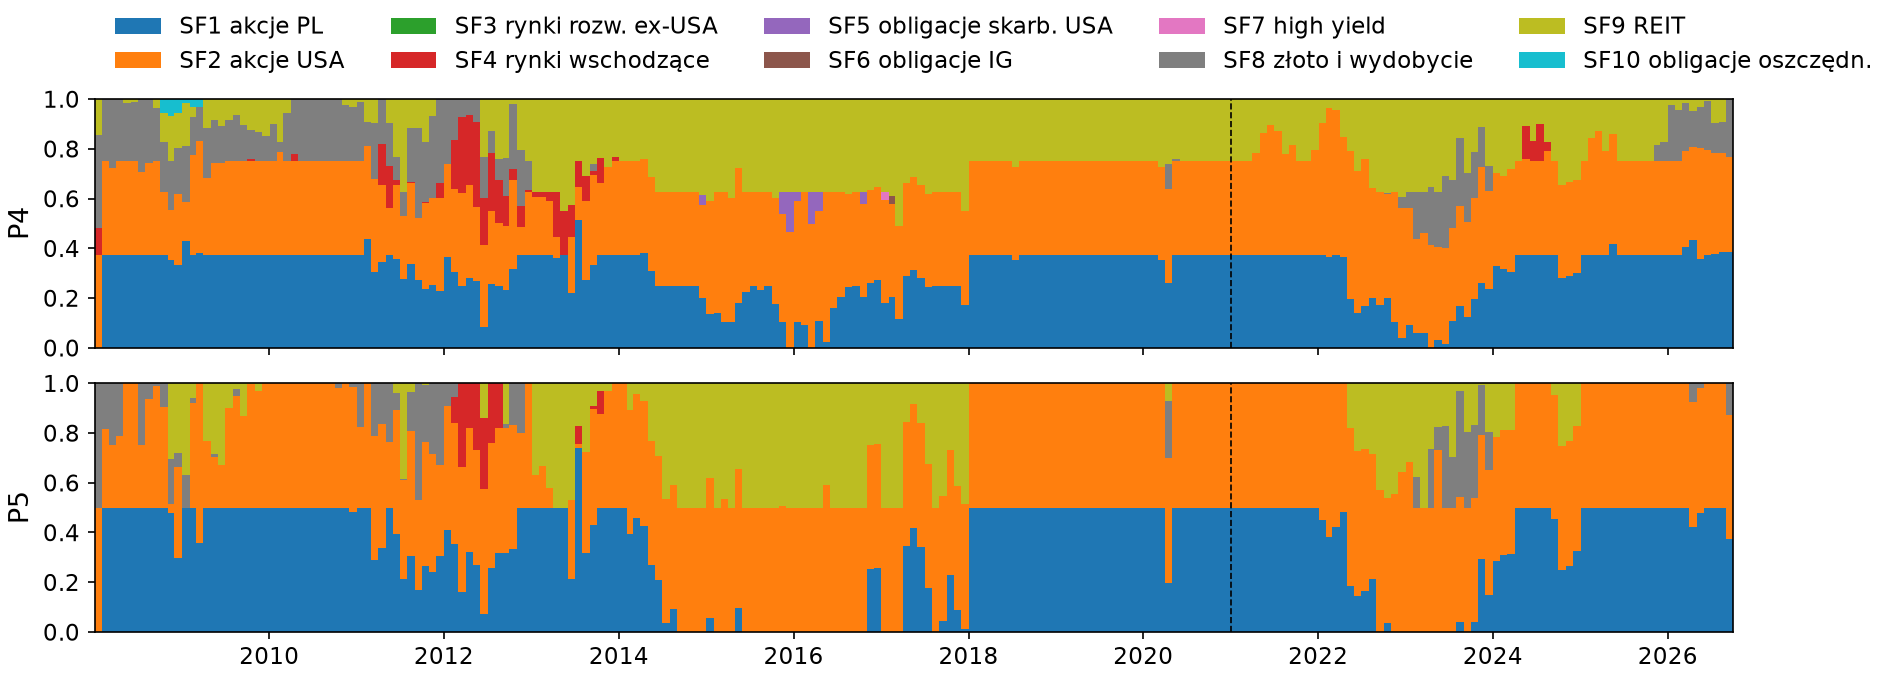
\includegraphics[width=\textwidth,height=.66\textheight,keepaspectratio]{portfolio_W_P4-P5.png}\par
\raggedright\smallskip
{\small Przy niższej awersji do ryzyka portfel koncentruje się w akcjach
  (SF1, SF2) i REIT (SF9). Udział SF1 ogranicza limit \(u_k\) wynikający z \(c_{LT}\).}
\source{https://github.com/michalmarchwiak/bsc-project/blob/main/pipelines/composition_figures.py}
       {Kod wykresu: pipelines/composition\_figures.py}
\end{frame}

% ------------------------------------------------------------ pasted (3)
\begin{frame}{Czy prognozy ryzyka sprawdziły się poza próbą?}

\begin{enumerate}
  \item Przed rebalansowaniem zapisujemy prognozy VaR i ES,
        korzystając z danych dostępnych przed decyzją.
  \item Po zakończeniu okresu porównujemy prognozy
        z rzeczywistą stratą portfela.
\end{enumerate}

\begin{block}{Wynik dla miesięcznego VaR 97,5\%}
\centering
\begin{tabular}{lrr}
\toprule
Próba & Oczekiwane przekroczenia & Średnio zaobserwowane \\
\midrule
Kalibracja (156 miesięcy) & 3,9 & 14,5 \\
Hold-out (69 miesięcy)   & 1,7 & 6,1 \\
\bottomrule
\end{tabular}
\end{block}

W hold-oucie straty przekraczały prognozowany próg częściej,
niż wynikało z poziomu ufności. Około 53\% przekroczeń
przypadło na 2022 r.

\source{https://github.com/michalmarchwiak/bsc-project/blob/main/artifacts/reports/backtest_summary.md}
       {Raport przebiegu 7d0ff370e76f}
\end{frame}

\end{document}
